\subsection{Tool Usage}

% CJM: Moving this figure here to allow reader to follow the process of the mrstudr tool

%!TEX root=../icsme2016-mrstudyr.tex

\newcommand{\mx}[1]{\mathbf{\bm{#1}}} % Matrix command
\newcommand{\vc}[1]{\mathbf{\bm{#1}}} % Vector command

% Define the layers to draw the diagram
\pgfdeclarelayer{background}
\pgfdeclarelayer{foreground}
\pgfsetlayers{background,main,foreground}

% Define block styles used later

\tikzstyle{sensor}=[draw, fill=black!5, text width=15em,
text centered, minimum height=2.5em,drop shadow]
\tikzstyle{smallsensor}=[draw, fill=black!5, text width=4em,
text centered, minimum height=2.5em,drop shadow]
\tikzstyle{box}=[draw, text width=8em,
text centered, minimum width=17.5em, minimum height=3.5em]
\tikzstyle{calc}=[draw, fill=black!5, text width=2.5em,
text centered, rounded corners, minimum height=2.5em,drop shadow]
\tikzstyle{circle}=[draw, ellipse, fill=black!5, text width=11em,
text centered, minimum height=2.5em, drop shadow]
\tikzstyle{mr}=[draw, fill=black!20, text width=5em,
text centered, minimum height=17em, minimum width = 18em, drop shadow]

% Define distances for bordering
\def\blockdist{1.5}
\def\edgedist{2.5}

\begin{figure}[t]

  \vspace{-.75em}

  \centering
  % SIMPLE
  \begin{tikzpicture}[thick,scale=0.85, every node/.style={scale=0.85}]
    \node [mr] at (0, 0) (mr) {};
    \node [circle] at (0, 3.7) (md) {Original Data};
    \node [sensor] at (0, 2.25) (r) {Reduction Techniques};
    \node [circle] at (0, 0.75) (rmd) {Cumulated Reduced Data};
    \node [sensor] at (0, -0.75) (ra) {Efficiency \& Effectiveness Analysis};
    \node [box] at (0, -2.25) (box) {};
    \node [calc] at (-2.25, -2.25) (ms) {MS};
    \node [calc] at (-0.75, -2.25) (err) {Red.};
    \node [calc] at (0.75, -2.25) (corr) {Corr.};
    \node [calc] at (2.25, -2.25) (err) {Err.};
    \node [sensor] at (0, -3.75) (he) {Human Examination};
    \node [circle] at (0, -5.25) (pr) {Policy Recommendation};

    \path [draw, ->] (md.south) -- node [above] {}
      (r.90);
    \path [draw, ->] (r.south) -- node [above] {}
      (rmd.90);
    \path [draw, ->] (rmd.south) -- node [above] {}
      (ra.90);
    \path [draw, ->] (ra.south) --  node [above] {}
      (box.90);
    \path [draw, ->] (box.south) --  node [above] {}
      (he.90);
    \path [draw, ->] (he.south) -- node [above] {}
      (pr.90);
  \end{tikzpicture}

  \caption{\label{fig:mrstudyr}The inputs and outputs of the \mr~tool.}

  \captionpara{0.5}{0.9}{0.5}{In this figure, the dark square represents the \mr~tool and its constituent parts, a
    rectangle stands for a process, a rectangle with rounded edges is a calculation performed by \mr, and an ellipse
  symbolises a process output.}

  \vspace{-1.8em}
\end{figure}



% CJM: I think we should move 'data' to the same line as the function call

Releasing an R tool via a package makes installing and loading the tool a matter of a few commands,
but does not guarantee tool usability. \mr~was designed to be simplistic, yet perform stringent
empirical analyses on mutant reduction techniques. To display the results from \mr~analysing mutant
reduction strategies for the testing of real-world database schemas, the following commands will be
tailored toward the data that we collected from performing mutation testing. The collected data can
be read in via the following: {\small\texttt{data <- read\_data("sqlite-avmdefaults.dat")}}. This
function expects the data to be located in the \texttt{inst/extdata} folder and stored as a
comma-separated value file.

% CJM: I noticed in section 2.C (Conducting Experiment Campaigns) that it already explains that mrstudyr
% focuses on mutant sampling. Therefore, I am going to remove the sentences in this section restating
% this fact. These sentences are commented-out immediately follow this comment.

% Currently, the two most common sub-techniques of mutant sampling are performed using the following:
% \texttt{analyse\_random\_sampling(data)} and \texttt{analyse\_across\_operators(data)},
% for random sampling and sampling across operators, respectively.

% CJM: Additionally, the attributes of the data that I describe are specific to mutant sampling. I will
% remove these attributes.

% CJM: Is including the following statement entirely necessary? I removed it for now.

% Sample output from the \texttt{analyse} function is provided in the accompanying README file on the
% tool's GitHub page~\cite{tool}.

The reduction techniques, reffered to in Figure~\ref{fig:mrstudyr}, are performed following the provision
of mutant data collected from mutation testing --- the ``Original Data'' --- to \mr. Using \mr~to perform
reduction techniques is a single command: \texttt{analyse(data)}. Each reduction technique performed by
the \texttt{analyse} function in \mr, returns reduced data which is then cumulated into a data set, shown
in Figure~\ref{fig:mrstudyr}, containing the data from all of the reduction approaches. This data includes
the trial, the total number of mutants analysed, the number of killed mutants, the generation time of each
mutant and the mutation scores for the reduced and original data. After performing the reduction techniques,
their efficiency and effectiveness is evaluated based on four calculations on the cumulated reduced data in
the ``E \& E Analysis'' phase.

% CJM: I want to present the evaluation metrics of efficiency and effectiveness, then define them, then finally,
% how to perform them with mrstudyr.
The evaluation calculations in E \& E analysis --- and their respective abreviations --- are: mutation score
(MS), reduction in creation cost (Red.), correlation (Corr.), and error (Err.). The mutation score is calculated
by dividing the number of killed mutants by the total number of mutants~\cite{wong1995reducing}. The reduction
in creation cost for a set of mutants is the cost of the reduced set subtracted from the cost of the original set,
divided by the cost of the original set. The original and reduced sets' mutation score correlation is calculated
using Kendall's~\taub, supported by the ``Kendall'' R package~\cite{mcleod2015kendall}. Finally, the error --- both
MAE and RMSE --- between the original and reduced sets' mutation score is calculated using the existing ``Metrics''
R package~\cite{metrics}.

The aforementioned metrics, with the exception of calculating correlation, are calculated by a single function
in \mr~: \texttt{analyse\_calculations(data)}. Where the input to \texttt{analyse\_calculations} is the cumulated
reduced data, displayed in Figure~\ref{fig:mrstudyr}, from performing the reduction techniques and returns a data
set with the values of the respective calculation. To calculate correlation, the \texttt{analyse\_correlation(data)}
function is used. Where the input data to this function is again the cumulated reduced data and the output is a
data set containing only the correlation values between the reduced and original mutation scores. The usability of
\mr~is supported by requiring experimenters to only call two functions to analyse the efficiency and effective of
reduction techniques.

% CJM: removed this paragraph because I no longer think that it is needed and to save space for preliminary study
% Additionally, the \texttt{analyse\_calculations} function can be used to calculate the
% efficiency and effectiveness for any number of reduction approaches; it is not structurally
% limited to a single reduction method. As input, the \texttt{analyse\_calculations} function
% expects the dataframe returned from performing a reduction approach.

The ``Human Examination'' phase, displayed in Figure~\ref{fig:mrstudyr}, still requires use of \mr~for clearly
visualising the trends in the data collected from the E \& E analysis. The \mr~tool takes advantage of the work
of Hadley Wickham with widely-used graphing package \texttt{ggplot2}~\cite{ggplot2}. All of the visualisation
functions provided by \mr~and their output can be found on the GitHub page~\cite{tool}. These visualisations
will help human examiners to construct a policy recommendation as to which reduction technique should be used
for the specific domain and data under observation.

\begin{figure}[!t]

  \centering
  \hspace*{-1em}

  \begin{minipage}{4in}
    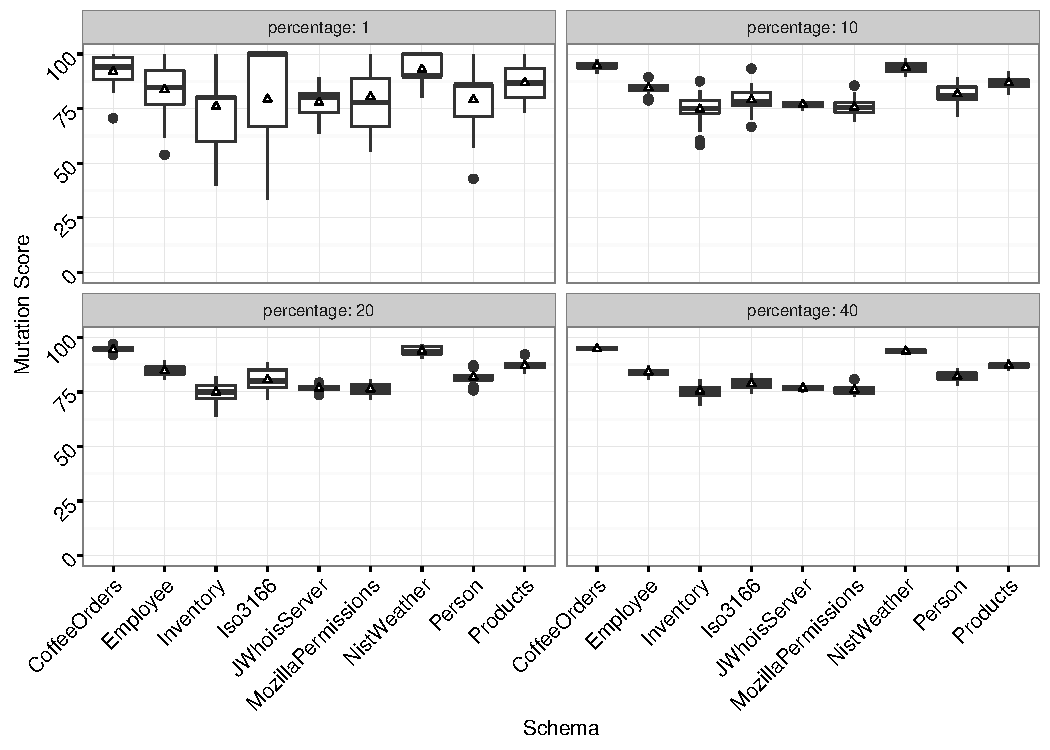
\includegraphics[scale = 0.5]{graphs/schema_vs_ms.pdf}
  \end{minipage}

  \caption{\label{fig:graph}Graph displaying mutation scores for database schemas.}

  \vspace{-1.8em}

\end{figure}

